\section{Independent-test CTR comparisons}
\label{app:ctr-plots}
The following figures collect the model-wise independent-test CTR comparisons
for both waveform modes and input windows. Corresponding numerical results and
uncertainty estimates are provided in Section~\ref{sec:results-tables}.

\subsection{UC board}
\begin{figure*}[p]
\centering
\begin{subfigure}[t]{0.49\textwidth}
\centering
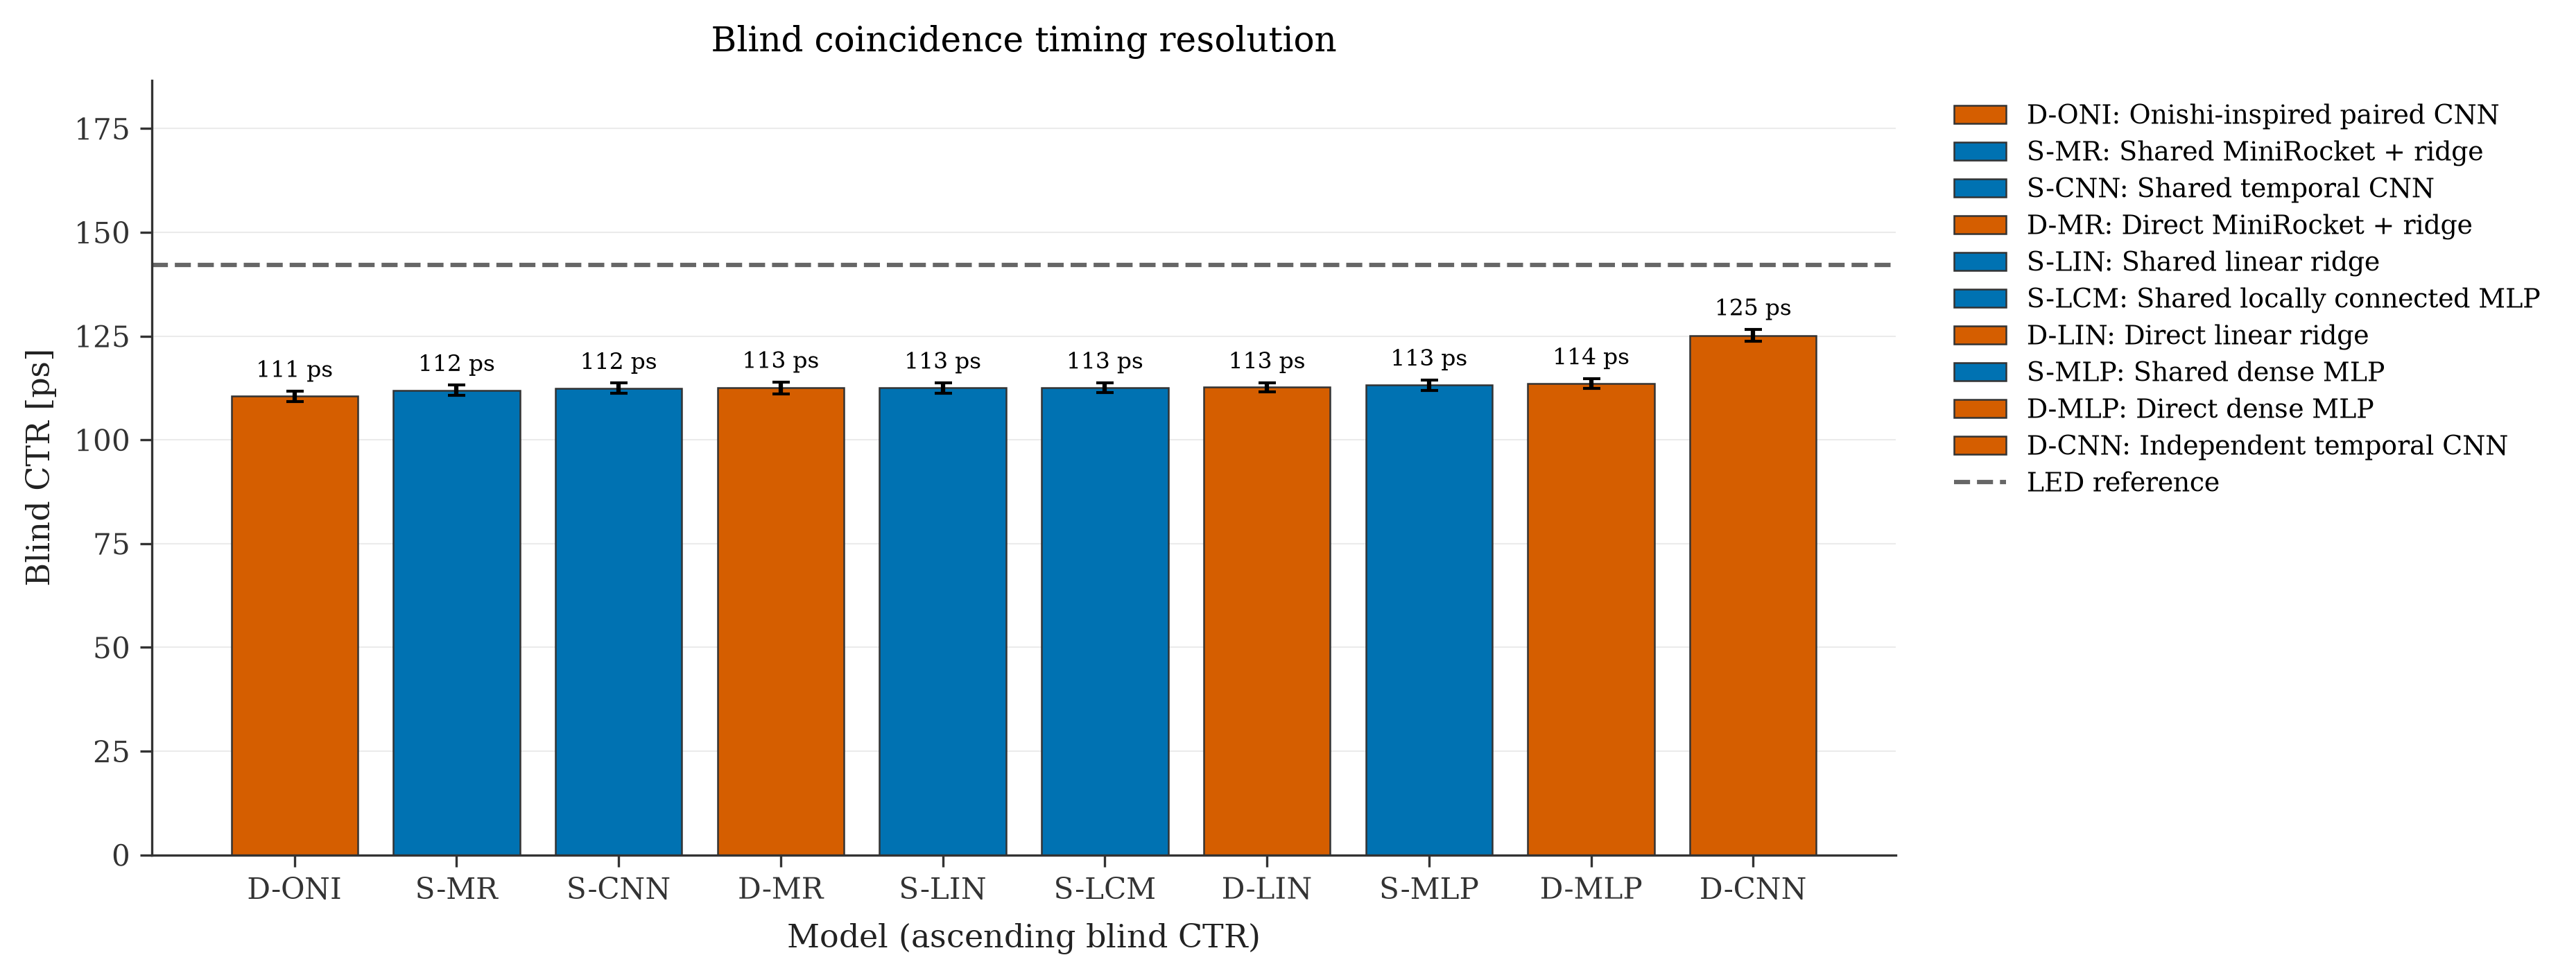
\includegraphics[width=\linewidth]{figures/results/UC/UC_energy_onishi_blind_ctr.png}
\caption{Energy, Onishi-inspired window.}
\label{fig:uc-energy-onishi-ctr}
\end{subfigure}\hfill
\begin{subfigure}[t]{0.49\textwidth}
\centering
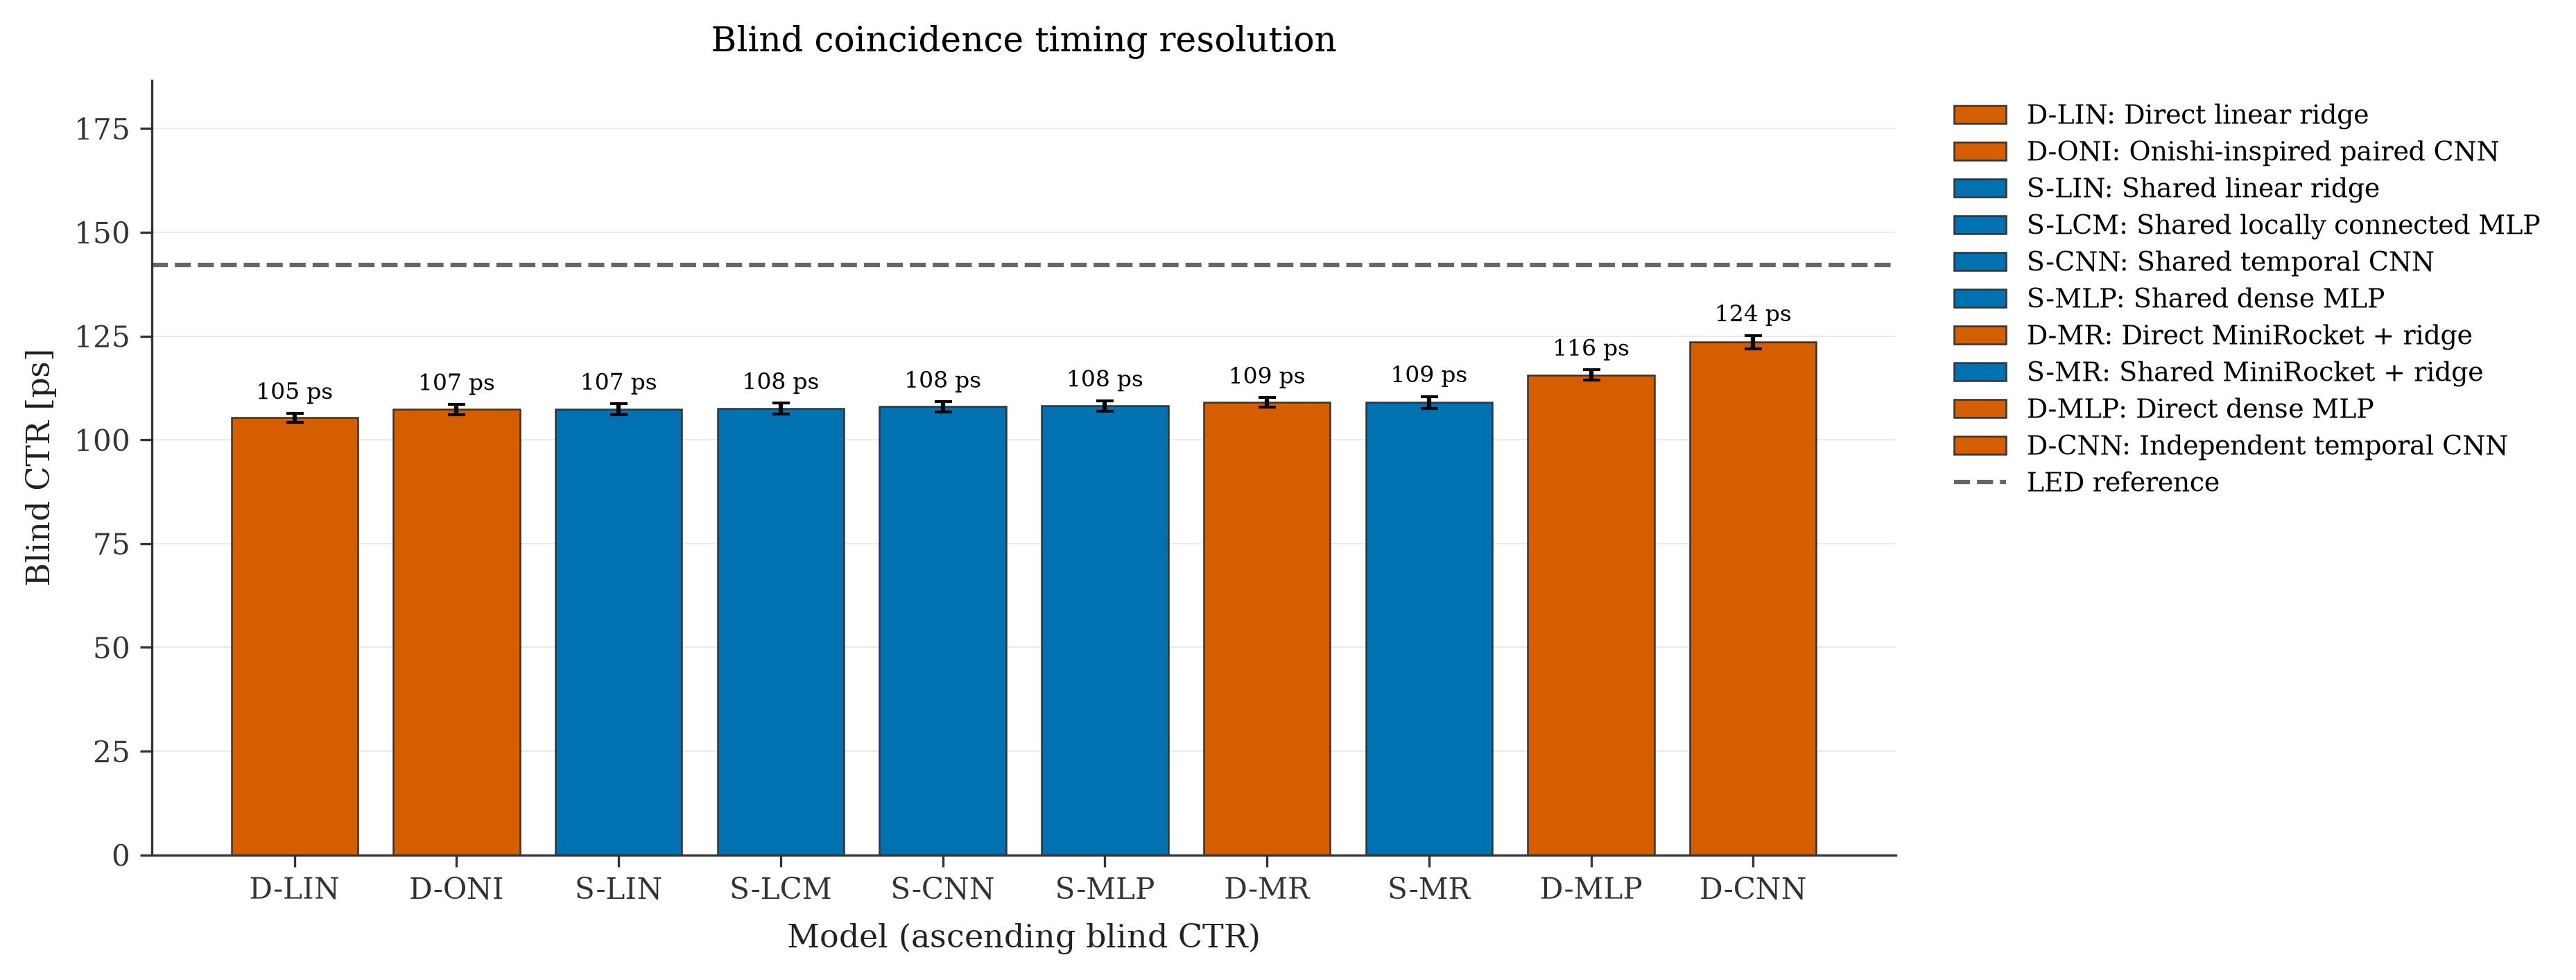
\includegraphics[width=\linewidth]{figures/results/UC/UC_energy_wide_blind_ctr.png}
\caption{Energy, wide window.}
\label{fig:uc-energy-wide-ctr}
\end{subfigure}

\medskip
\begin{subfigure}[t]{0.49\textwidth}
\centering
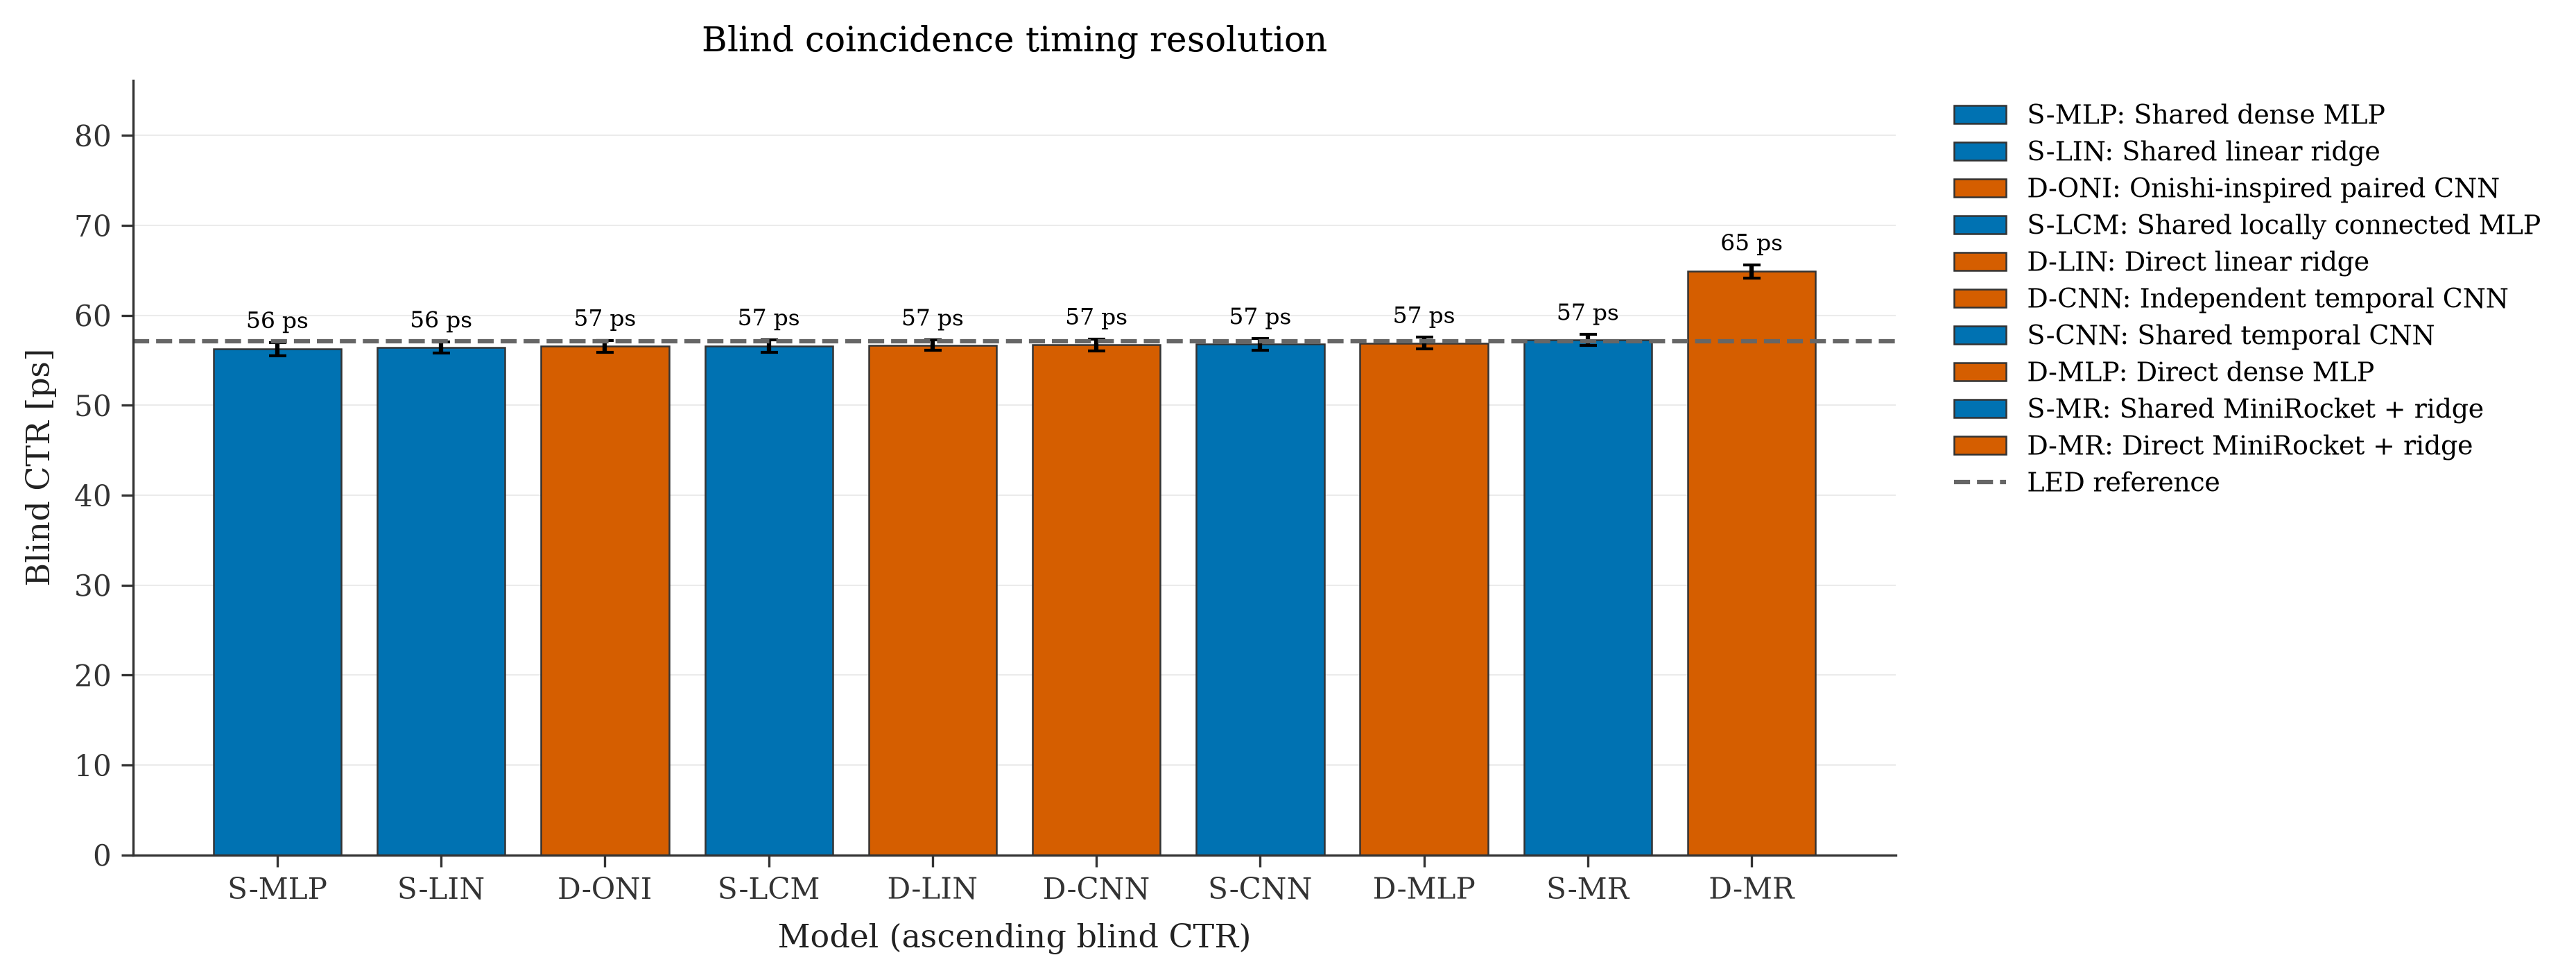
\includegraphics[width=\linewidth]{figures/results/UC/UC_timing_onishi_blind_ctr.png}
\caption{Timing, Onishi-inspired window.}
\label{fig:uc-timing-onishi-ctr}
\end{subfigure}\hfill
\begin{subfigure}[t]{0.49\textwidth}
\centering
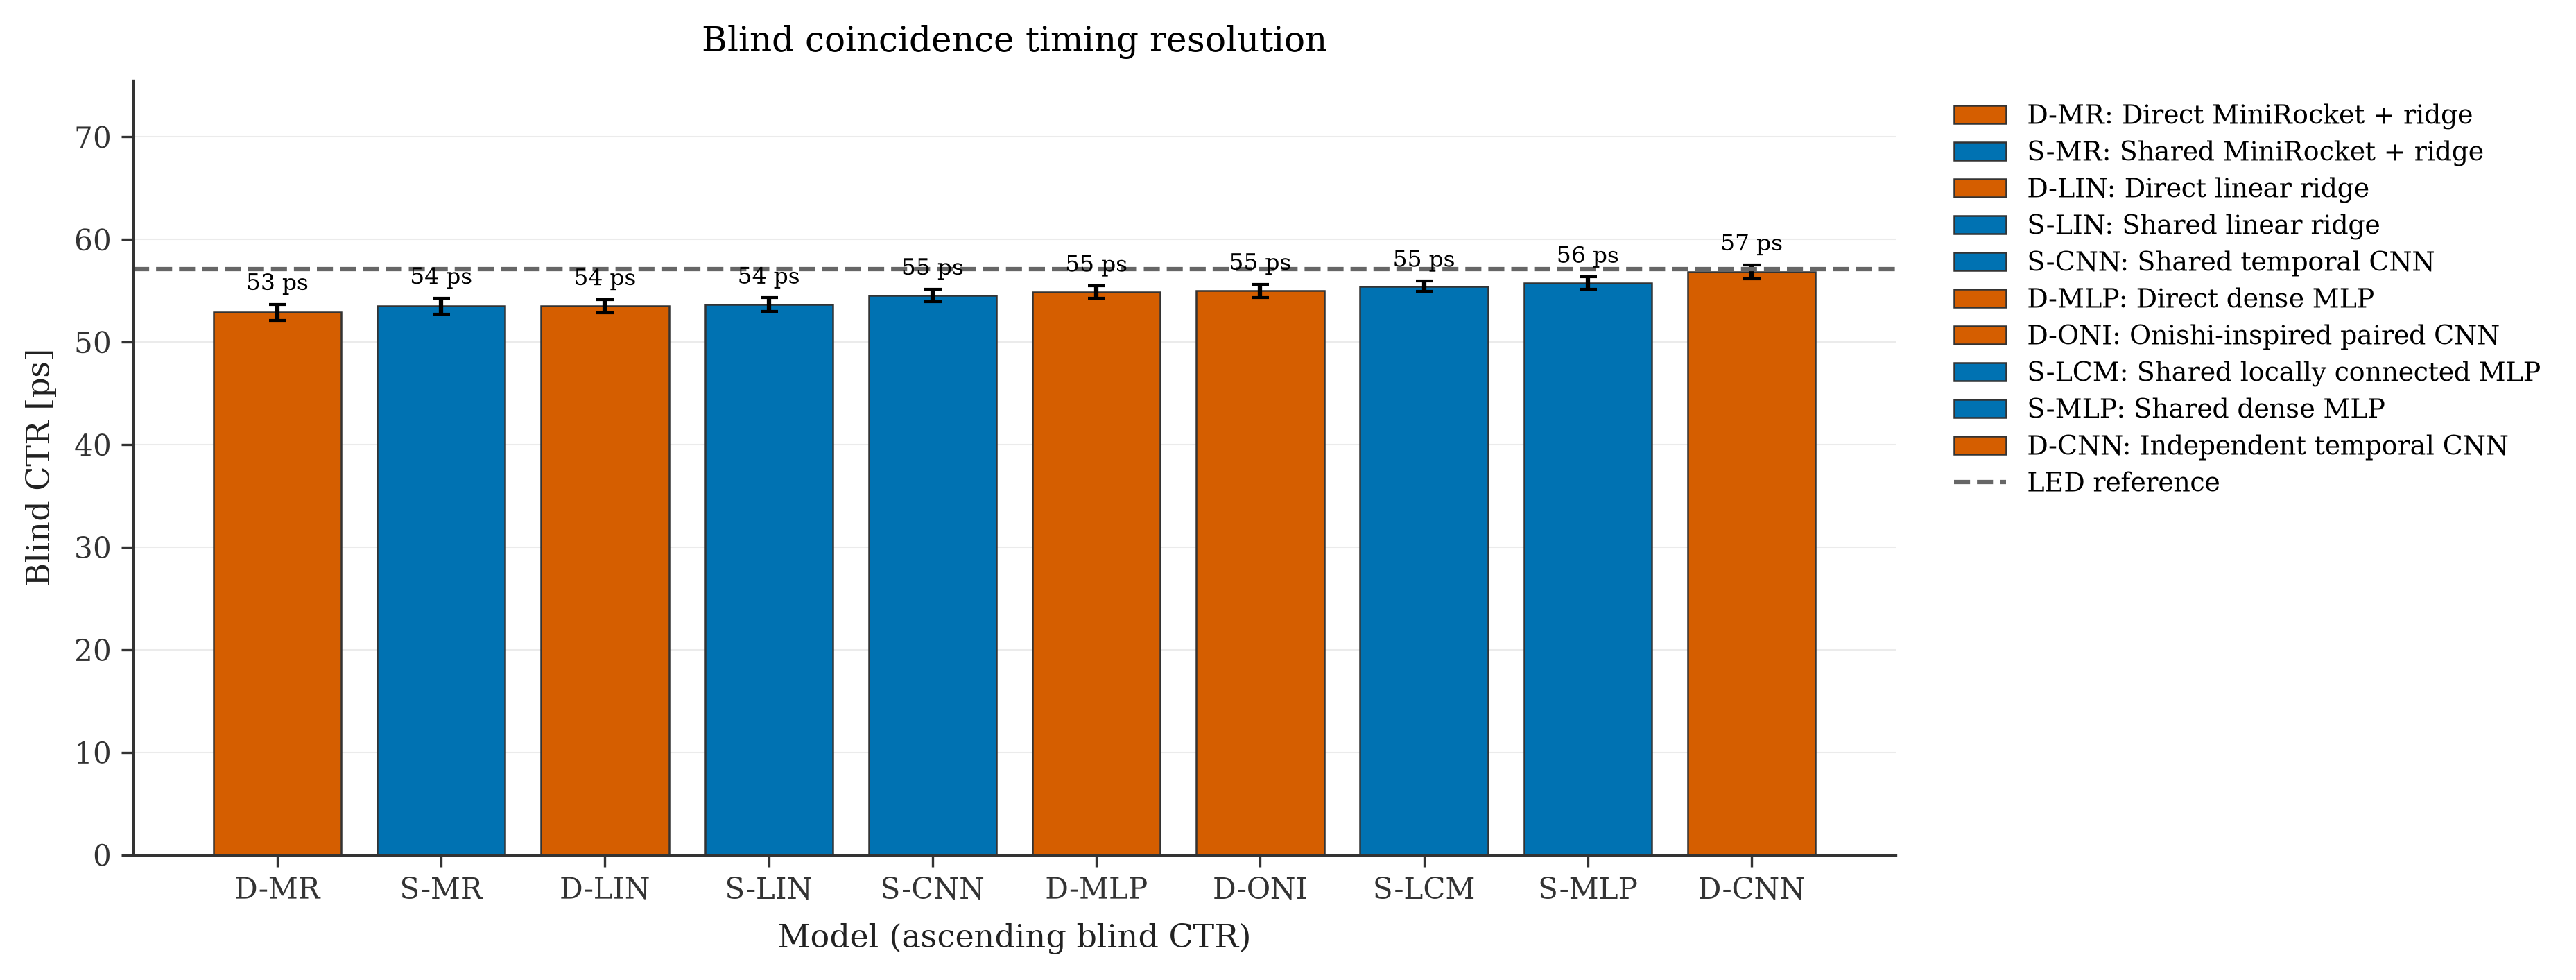
\includegraphics[width=\linewidth]{figures/results/UC/UC_timing_wide_blind_ctr.png}
\caption{Timing, wide window.}
\label{fig:uc-timing-wide-ctr}
\end{subfigure}
\caption{UC board: independent-test CTR for the compared estimators. The dashed
line denotes the LED reference and error bars indicate bootstrap standard
deviations.}
\label{fig:uc-ctr-comparison}
\end{figure*}

\subsection{FBK board}
\begin{figure*}[p]
\centering
\begin{subfigure}[t]{0.49\textwidth}
\centering
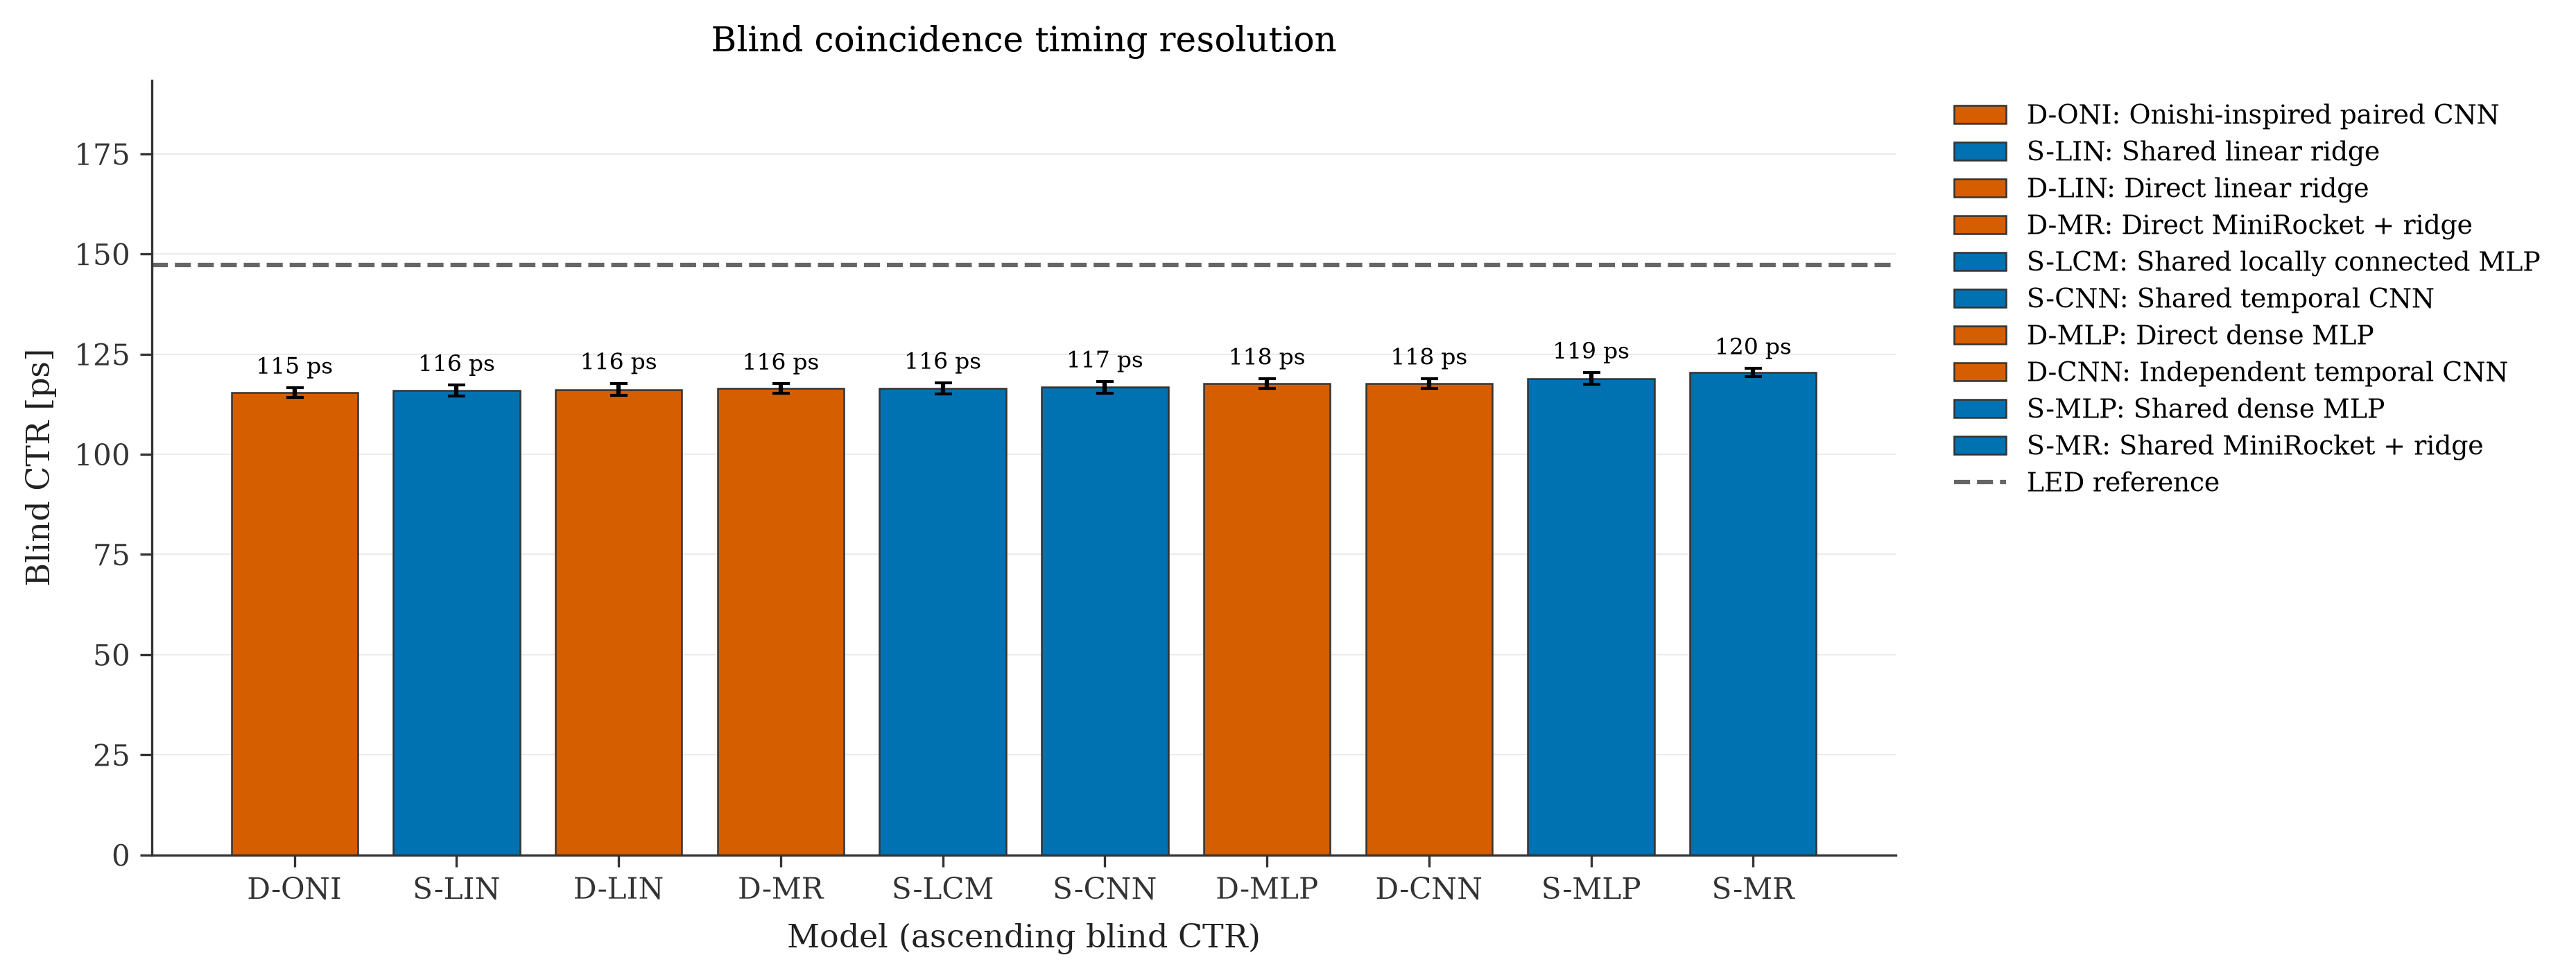
\includegraphics[width=\linewidth]{figures/results/FBK/FBK_energy_onishi_blind_ctr.png}
\caption{Energy, Onishi-inspired window.}
\label{fig:fbk-energy-onishi-ctr}
\end{subfigure}\hfill
\begin{subfigure}[t]{0.49\textwidth}
\centering
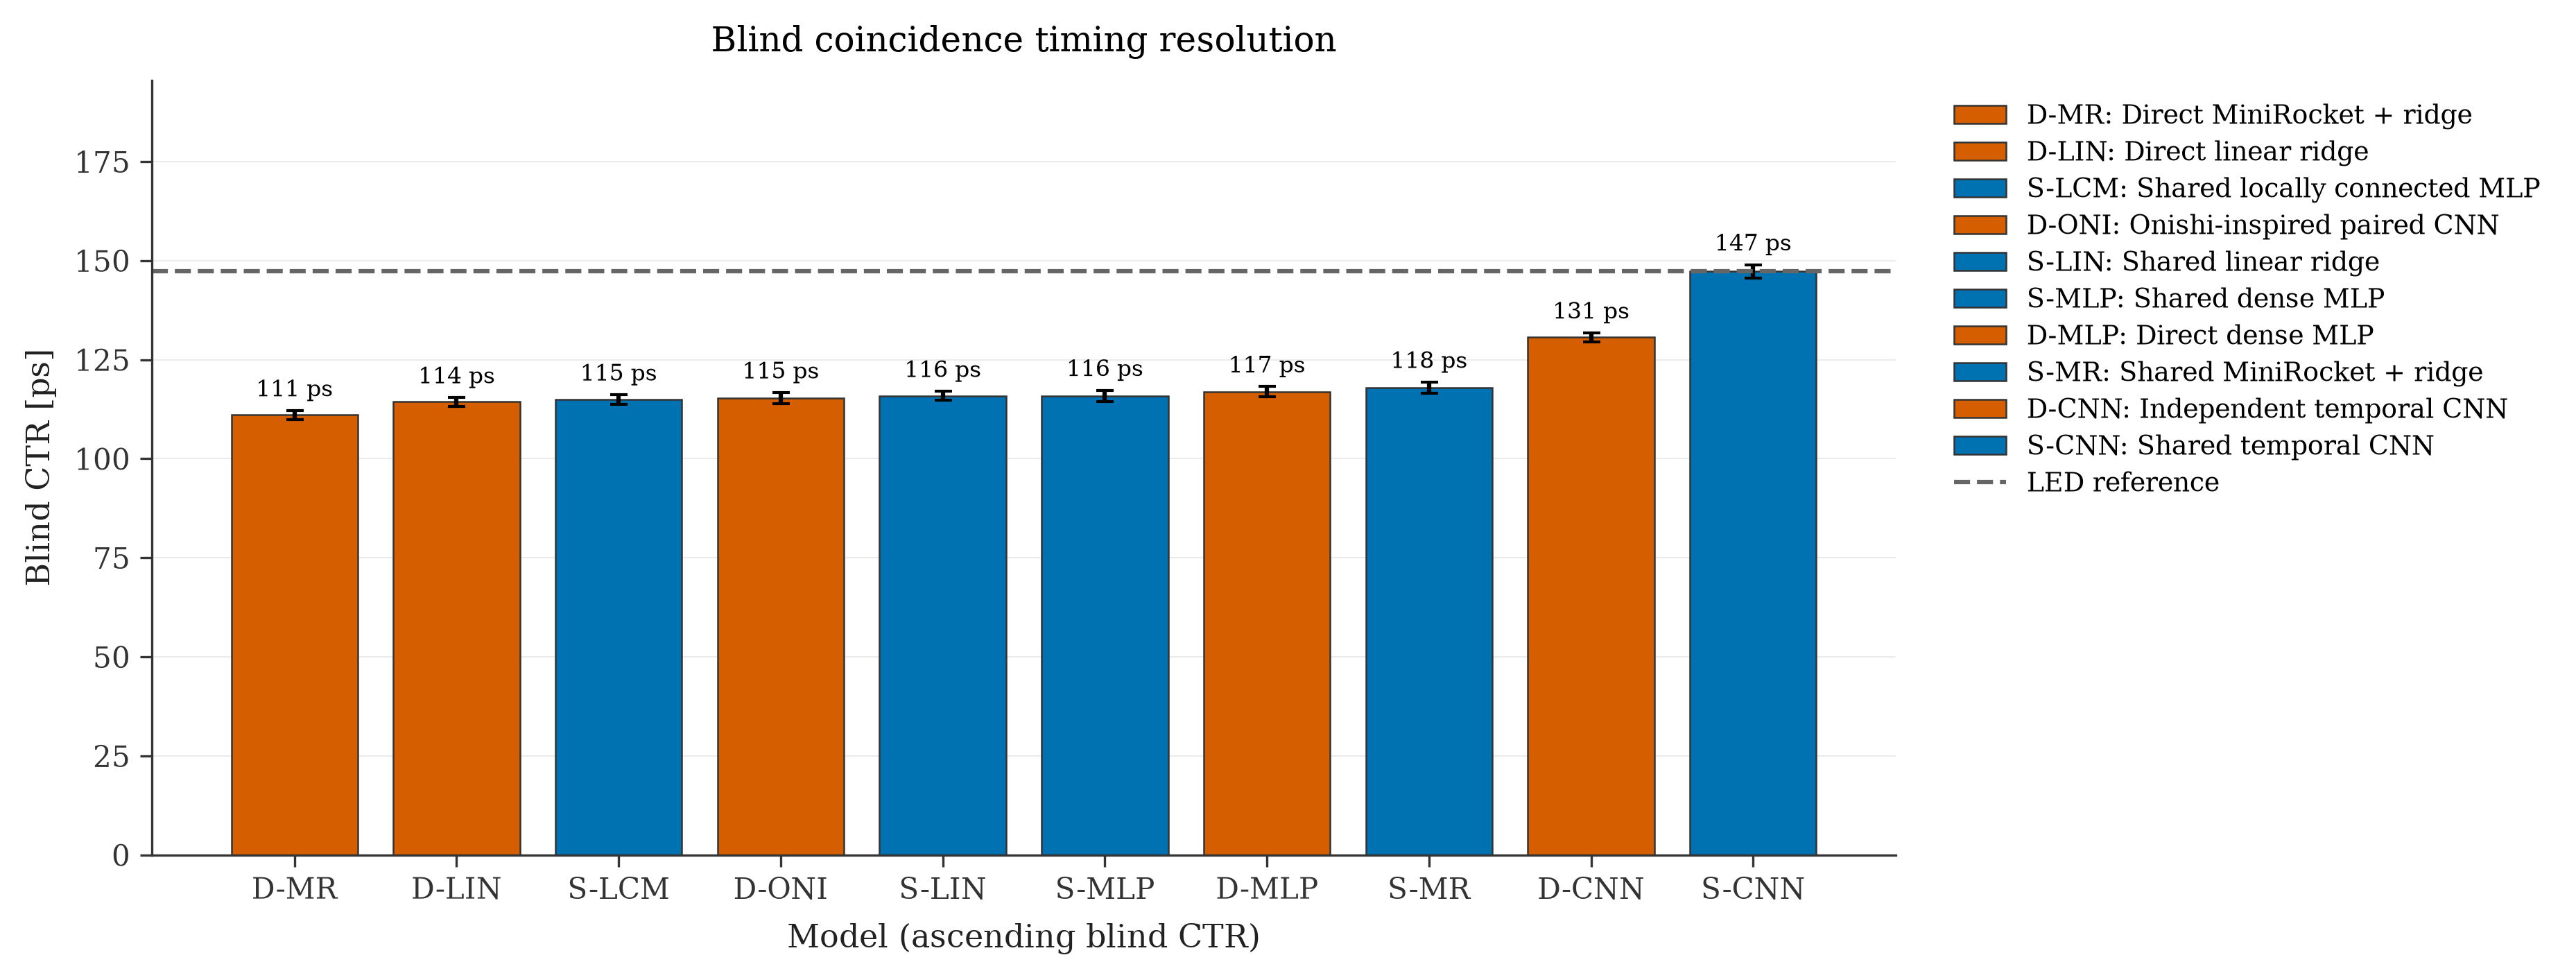
\includegraphics[width=\linewidth]{figures/results/FBK/FBK_energy_wide_blind_ctr.png}
\caption{Energy, wide window.}
\label{fig:fbk-energy-wide-ctr}
\end{subfigure}

\medskip
\begin{subfigure}[t]{0.49\textwidth}
\centering
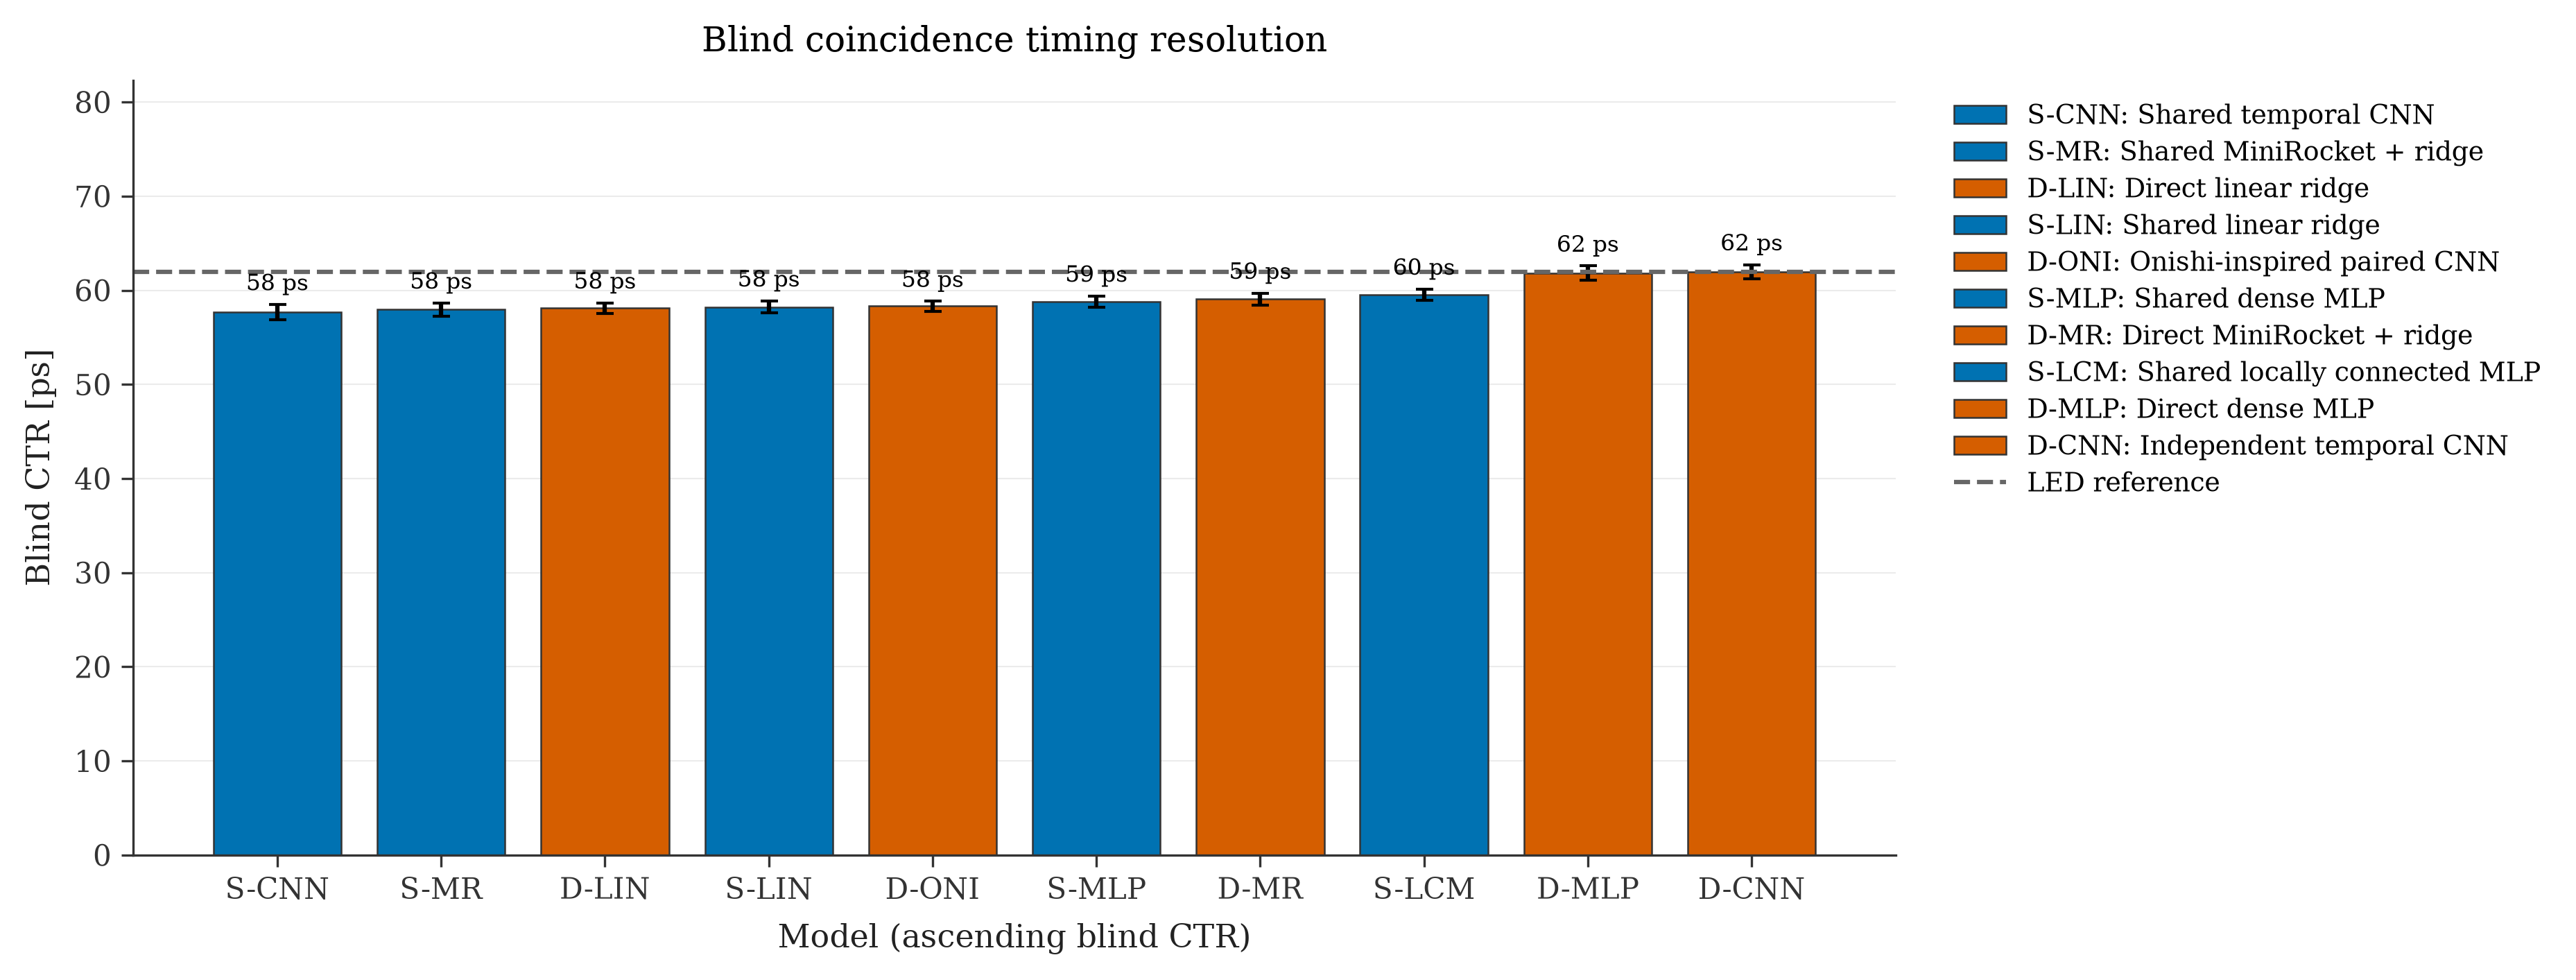
\includegraphics[width=\linewidth]{figures/results/FBK/FBK_timing_onishi_blind_ctr.png}
\caption{Timing, Onishi-inspired window.}
\label{fig:fbk-timing-onishi-ctr}
\end{subfigure}\hfill
\begin{subfigure}[t]{0.49\textwidth}
\centering
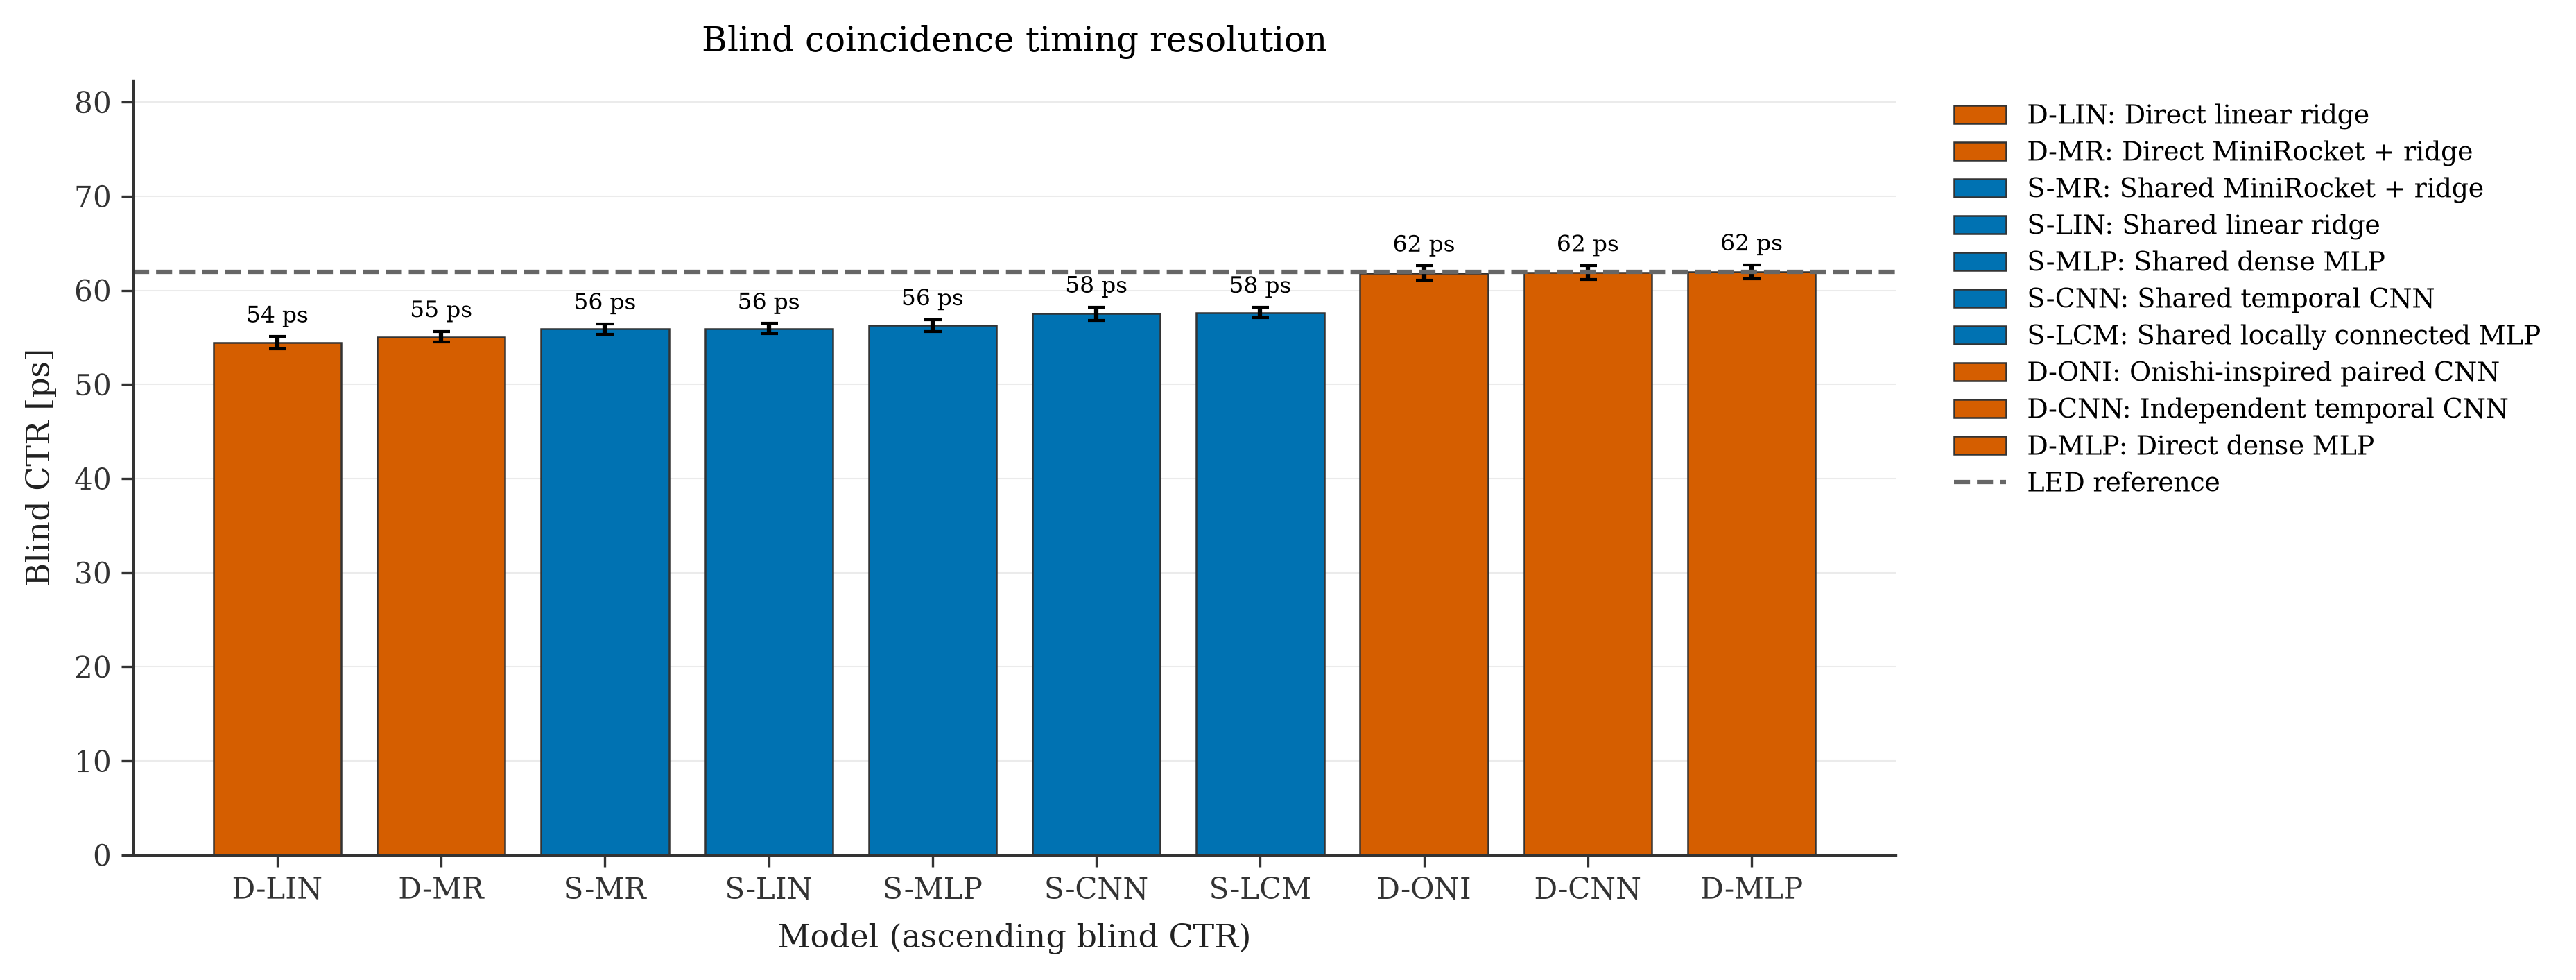
\includegraphics[width=\linewidth]{figures/results/FBK/FBK_timing_wide_blind_ctr.png}
\caption{Timing, wide window.}
\label{fig:fbk-timing-wide-ctr}
\end{subfigure}
\caption{FBK board: independent-test CTR for the compared estimators. The dashed
line denotes the LED reference and error bars indicate bootstrap standard
deviations.}
\label{fig:fbk-ctr-comparison}
\end{figure*}
